\documentclass[tikz,border=9pt]{standalone}
\usepackage{amsmath,amssymb}
\usetikzlibrary{arrows.meta,positioning,calc}
\begin{document}
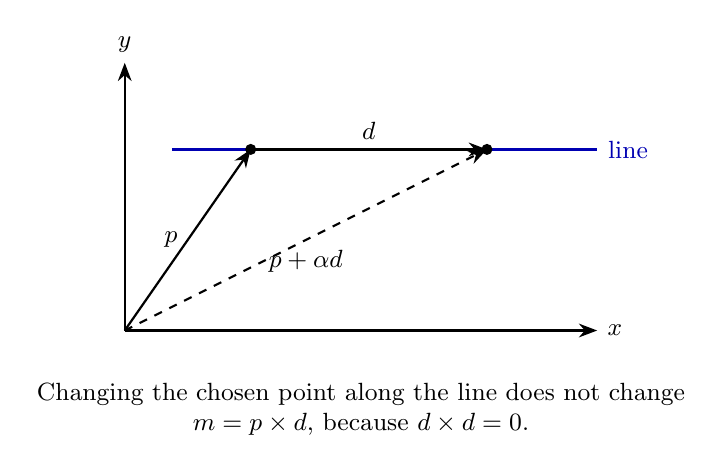
\begin{tikzpicture}[font=\small,arr/.style={-{Stealth},thick},box/.style={draw=blue!55!black,rounded corners,fill=blue!4,align=center,text width=2.9cm,minimum height=1.05cm}]

\coordinate (O) at (0,0);\coordinate (p) at (1.6,2.3);\coordinate (q) at (4.6,2.3);
\draw[arr] (O)--(6,0) node[right]{$x$};\draw[arr] (O)--(0,3.4) node[above]{$y$};
\draw[very thick,blue!70!black] (.6,2.3)--(6,2.3) node[right]{line};
\draw[arr,thick] (O)--(p) node[midway,left]{$p$};\draw[arr,thick] (p)--(q) node[midway,above]{$d$};
\draw[arr,dashed] (O)--(q) node[midway,below]{$p+\alpha d$};
\fill (p) circle(2pt);\fill (q) circle(2pt);
\node[align=center] at (3,-1){Changing the chosen point along the line does not change\\$m=p\times d$, because $d\times d=0$.};

\end{tikzpicture}
\end{document}
